\documentclass[10pt,a4paper]{article}
\usepackage{amsmath}
\usepackage{float}
\usepackage{graphicx}
\title{Advanced Computer Architecures notes}
\author{Elia Ravella}
\begin{document}
	\begin{titlepage}
		\maketitle
	\end{titlepage}
	
	\tableofcontents
	\clearpage
	
	\clearpage \part{Introduction}
		\section{Taxonomy of Computer Architectures}
			\subsection{Flynn Taxonomy}
				Flynn defined four categories to group computing architectures. This so called taxonomy helps system architects to distinguish among possible models of processors or system themselves. 
				\begin{enumerate}
					\item SISD: Single Instruction Single Data, uniprocessor systems;
					\item MISD: Multiple Instructions Single Data, no commercial application;
					\item SIMD: Single Instruction Multiple Data, low overhead, used in custom integrated circuits;
					\item MIMD: Multiple Instruction Multiple Data, off the shelf micros
				\end{enumerate}
				SISD is the simplest and most diffuse model of computation, one data stream in input and a \emph{single} instruction executed per istant of time. SIMD introduces parallelism in a vector fashion: multiple processes execute a single instruction (the \emph{same} instruction) on different data elements. Another type of parallelism: MIMD. Just SIMD with multiple different instructions per instant.
				
	\clearpage \part{Performance and Cost}
		\section{Performance}
			\subsection{Evaluating performance}
				We need to distinguish between how to measure performance of a computer architecture and what impacts it without affecting performance. The amount of memory used is not a performance evaluator, but it affects performance in some way. The power consumed, the latency and the execution time are. To evaluate the performance of a CA I must use all the performance indicator and find the right tradeoff. Also, context! A CA is inserted in a context that bounds its scope, so the environment itself shapes the way performance is evaluated\\
				\emph{Every performance indicator} says something about the CA. So, the whole system must be evaluated with a \emph{whole set} of indexes that each tell a different thing about the system itself. This provides a full view of the system strenghts and weaknesses and highlights the things to optimize.
				
			\subsection{Quantifying the Design Process}
				"The frequent case" case: when designing a CA, the "frequent case" represents the set of conditions met \emph{the most times} during a standard computation run. Optimizing the standard case means optimizing \emph{singnificately} all the system behaviour. 
				
				\paragraph{Amdahl's Law}
					Amdahl's law describes the concept of the speedup as a function of execution time. The set of formulas that describes the law is
					\begin{equation}
						EXTIME_{new} = EXTIME_{old} \times [(1-Fraction_{enhanced}) + \frac{Fraction_{enhanced}}{Speedup_{enhanced}}]
					\end{equation}
					\begin{equation}
						SPEEDUP_{overall} = \frac{EXTIME_{old}}{EXTIME_{new}} = (1-Fraction_{enhanced} + \frac{Fraction_{enhanced}}{Speedup_{enhanced}})^{-1}
					\end{equation}
					and calculates the speedup of a system taking into account all his part, the speedupped one and the invariate one.\\
			
			\subsection{Indexes on performance}
				Overview of performance indicators and measurements.
				\begin{itemize}
					\item Instruction Count: the effective number of instructions executed. This is influenced also by the program we're trying to execute.
					\item Time per Cycle: the clock rate. OBVIOUSLY influenced by the hardware architecture.
					\item MIPS and MFLOPS indicates already a very \emph{program bound}-like perfomance indicator. They represents the number of integer/floating point operations that the architecture can carry out in a second. They're very synthetic indexes.
					\item CPI - Average CPI (clock per instruction) represents obviously the amount of clock cicles that are necessary to carry out a specific operation. The element that most impacts the CPI is the ISA: the alphabet we use shapes the words we can create. 
				\end{itemize}
				Notice how execution time is not present. That's because \emph{reducing execution time is the goal}, so execution time does not modify performance, it just \emph{represents} it. 
			
			\subsection{Benchmarking}
				Benchmarking is "running a fake program with the sole purpose to evaluate a system and find bottlenecks". It's a technical test. Workloading a CA means feeding it with a real work load to test what is a response to a non-syntethic stimulus.\\
				Benchmarking must be
				\begin{enumerate}
					\item representative: we need to benchmark the right aspects of the architecture we're testing.
					\item updated: old benchmark does not test the architecture well, because of the very architecture is changed and the benchmark is \emph{not anymore representative} because it's \emph{old}.
				\end{enumerate}
			
			\subsection{Energy, Power}
				Energy and power consumption are a "cost - like" performance indicator. The less the power, the less the cost of keep the architecture running, and tha's easy. Also, reducing the power consumed means \emph{reducing the power needed from a battery} and this impacts a lot in the mobile scenario. Energy per task is a good indicator for energy consumption. The power used by an architecture is influenced by a ton of factors, not least the TDP (thermal design power). Also architecture-bound aspects (clock rate, voltages, busses) influence power consumption \emph{heavily}.

	\clearpage \part{Pipelining}
		\section{MIPS architecture}
			Reference architecture for this course is MIPS.\\
			MIPS is a RISC architecture (Reduced Instruction Set Computer) this means that the only possible operation (that are very optimized) are basic operations. This kind of architecture is the opposite of CISC (Complex ISC) where more complex operation are supported at chip level.\\
			MIPS is a LOAD/STORE architecture. This means that data cannot come into the ALU from anywhere besides the CPU general purpose registers. MIPS uses 32-bit instructions that can be
			\begin{itemize}
				\item Register Register operations
				\item Register Immediate operations
				\item Branch operations
				\item Jump/Call operations
			\end{itemize}
			Operand lenght is 6-bit. We have 64 possible operations.\\
			
			\subsection{Assembly basics}
				We'll see three classes of MIPS instructions:
				\begin{itemize}
					\item ALU: add "reg target" "reg source" "reg source", or sub "reg target" "reg source" "immediate"
					\item LOAD/STORE: lw "reg target" "offset register" (load word)
					\item Branches/Jumps: classic bne or bge or jmp operations
				\end{itemize}
			
			\subsection{MIPS instruction execution}
				A fetch - decode - execute cycle in this architecture works this way:
				\begin{enumerate}
					\item Fetching the instruction means sending the PC content to the memory in order to access the memory location where the instruction is. Then, the PC is updated (PC + 4, each instruction take 32 bits).
					\item Decoding the instruction: in this phase a fixed-field operation is put in place to deconde the instruction itself, and the registers needed for the computation are read.
					\item Execute operation: the ALU calculates the result of the instruction supplied.
					\item Memory Access and Write Back phases: in these two phases the CPU takes care of the memory access (LOAD or STORE instructions) and the registers update.
				\end{enumerate}

				
			\subsection{MIPS Chip Architecture}
				\begin{figure}[H]
					\centering
					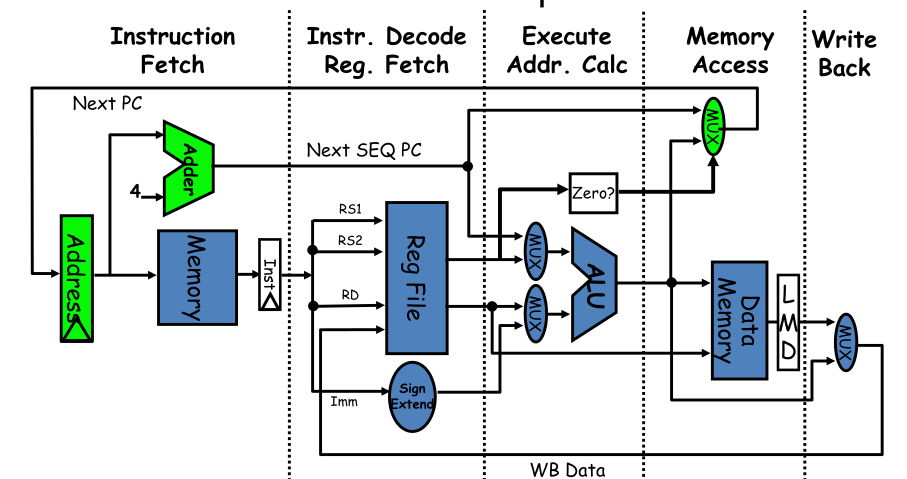
\includegraphics[width = \textwidth]{./images/MIPSDP.png}
					\caption{The MIPS data path with pipeline stages highlighted}
				\end{figure}
				
				\begin{figure}[H]
					\centering
					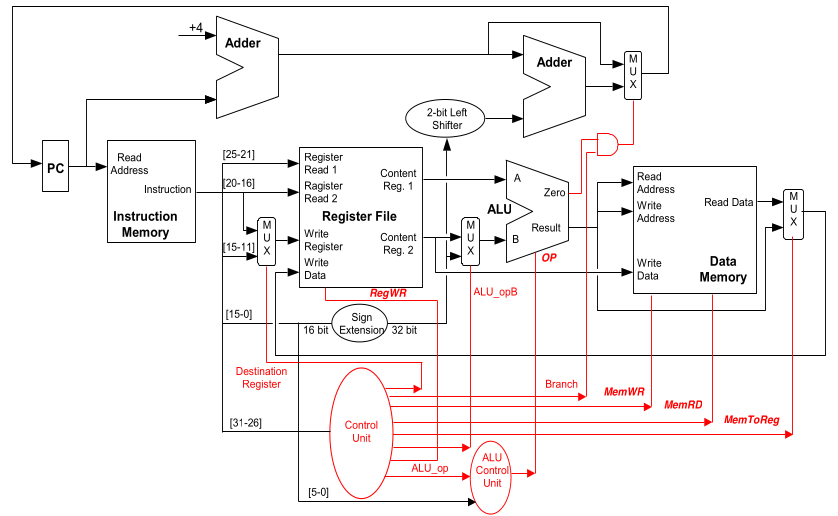
\includegraphics[width = \textwidth]{./images/MIPSCPU.png}
					\caption{The MIPS full CPU, data path integrated with control unit}
				\end{figure}
				
				\begin{figure}[H]
					\centering
					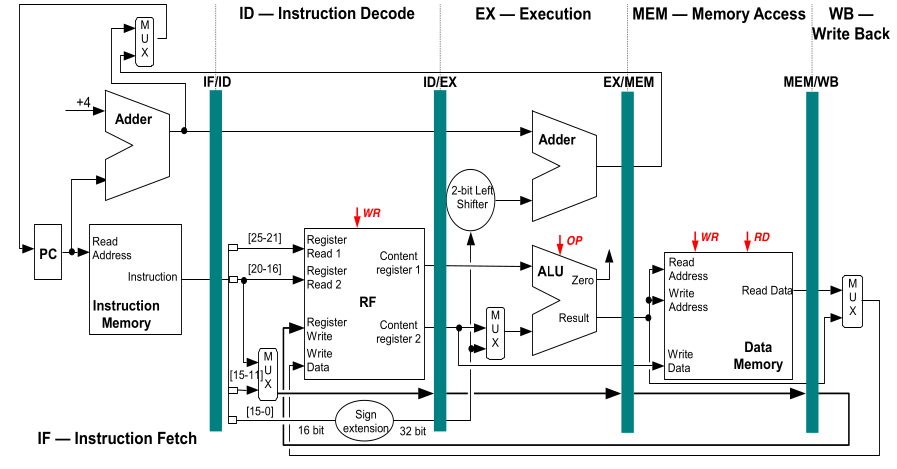
\includegraphics[width = \textwidth]{./images/MIPSCPUPIPELINED.png}
					\caption{Pipelined MIPS}
				\end{figure}
				
				
		\section{Data and Control}
			Every computer architecture is composed of 2 main parts: the one that computes data (datapath) and the one that controls the execution (control unit).
			
			\paragraph{Datapath}
				The datapath runs the house. All data pass through this module, and the registers here are used to pipeline operation.
			
			\paragraph{Control Unit}
				The CU guides the computations. It takes "run time decisions" in order to pilot execution of intructions. The registers here are architecture-specific.
				
			\paragraph{Memory}
				And memory? "Slow primary memory" is connected with the CPU (so DP + CU) by means of buses. The structure is similar to:
				\begin{figure}[H]
					\centering
					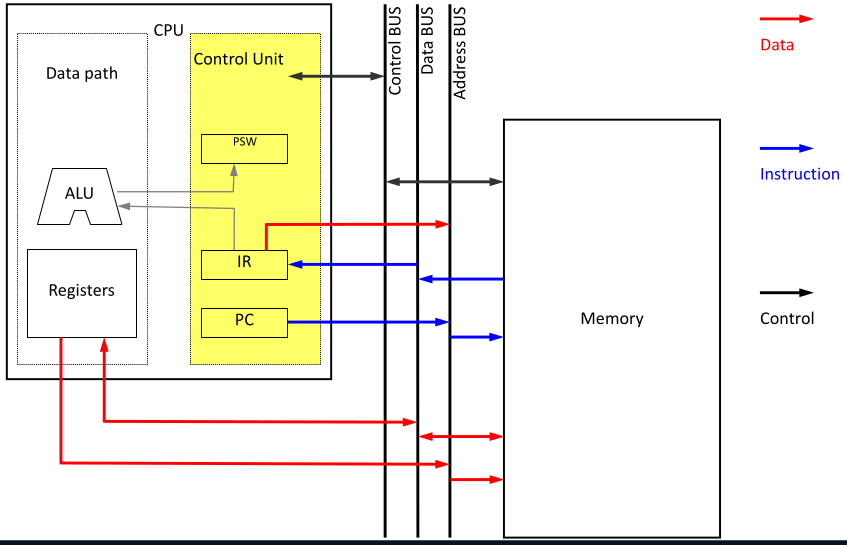
\includegraphics[width = \textwidth]{./images/ArchBuses.png}
				\end{figure}
				Things to be noted:
				\begin{enumerate}
					\item the datapath does not connect to the control path
					\item the control unit does not write on the data bus
				\end{enumerate}
				
		\section{Hazards}
			Pipelining is cool, parallele, throughput enhancing and overall faster. Does she have drawbacks? YES, hazards. Both the ID and the WB phases in the pipeline we have an access to the registers, that can overlap. This is usually overcome assigning (for example) rising edge of the clock to reading and falling edge to writing.\\
			But what are hazards? An hazard is generated by dependency between two instructions. Hazards can be classificated in
			\begin{enumerate}
				\item Structural hazards: the registers example. Different phases of the same pipeline access simoultaneously the same resource.
				\item Data hazards: attempting to \emph{reading the future}: accessing a piece of data that's not be computed yet. 
				\item Control hazards: making a decision basing on a condition \emph{not yet evaluated}.
			\end{enumerate}
			
			\subsection{Structural Hazards}
				The attempt to use the same mutual exclusive hardware resource at the same time. No structural hazards in the reference architecture (edge - based synchronization)
				
			\subsection{Data Hazards}
				Utilizing a piece of data that is not ready is called the condition of data hazard (or data conflict). This is generally generated by two (or more) consecutive instructions that generate and use the same value.\\
				We can further classify the types of data hazards:
				
				\paragraph{Read after Write} 
					conflicts are generated by two consecutive operations, the first writes a value and the second reads it. In a pipelined environment, this can cause problems. This is the most common hazard.\\
					This kind of conflicts can be handled at compilation time (the compiler itself detects a dependence of this kind and inserts delays in the execution ("bubbles" or "stalls") of the instructions to distanciate "enough" the read and write operation. The cost is incremented overhead and increased execution time. This approach can also be implemented \emph{at architecture level}. The difference is that compiler will delay instructions with NOP instructions, while at architecture level clock cycle are just "skipped".\\
					Another way to resolve this kind of conflicts is to reschedule instructions (taking advantage of the dependencies between them) in order to 
					\begin{enumerate}
						\item distanciate enough the write-read conflicts
						\item not inserting dead times
					\end{enumerate}
					Forwarding, instead, is the technique that "bypasses" the WB phase and makes available the result of the ALU evaluation directly in the pipeline. So additional EX-EX, MEM-EX, MEM-MEM, MEM-ID\footnote{The MEM-ID path is not needed at all if we introduce that same-cycle read write in the architecture.} paths are introduced in the architecture. This approach does not cover certain type of conflicts, like load - use hazards. This conflict, however, is the only one possible in the reference architecture: all the other data hazards are solved with the insertion of forwarding paths.
				
					\begin{figure}[H]
						\centering
						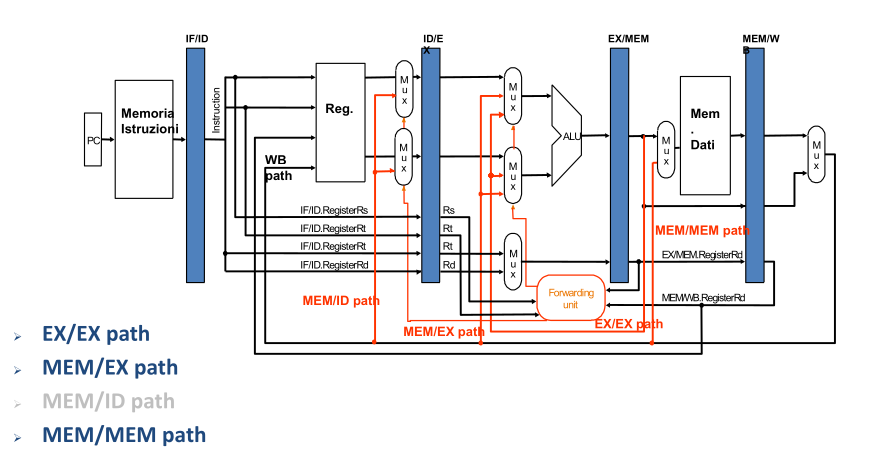
\includegraphics[width = \textwidth]{./images/forwarding.png}
						\caption{MIPSarchitecture with forwarding paths}
					\end{figure}
				
				\paragraph{Write after Write}
					It's a overwriting conflict. This is a problem when a WB stage of a instructions happens \emph{after} the WB phase of a \emph{following} instruction. This conflict can't happen in the reference architecture: all instructions takes 5 clock cycles.
					
				\paragraph{Write after Read}
					In a out-of-order scenario we can have a write operation of an instruction happens \emph{after} the read operation of an instruction \emph{preceding} her. This, again, is only possible when instructions can take more stages at executing than the instructions following them, so not possible in the reference architecture.
			
			\subsection{Control Hazards}
				Conditional instructions at assembly level are jumps (oversimplifying). The jump target address is computed just after the condition is evaluated (it can be PC + 1 or "TargetAddress").\\
				In the reference pipeline the PC is updated in the last pipeline stage, BUT we can skip the MEM phase because the PC is updated in the MEM phase itself. This kind of instructions (beq, bne) terminates after the MEM stage. This means that further instructions must wait for the MEM phase of the conditional statement in order to be fired, so \emph{at least 4 cycles}.\\
				The standard procedure to deal with this kind of instructions structure is to \emph{preload in the pipeline the "true" branch}, and then flush it if the condition is not met. Also, data forwarding reduces the number of stalls to be introduced: EX-ID path, for example, reduces the number of stalls from 3 to 2.
				
				\paragraph{Early Evaluation}
					What if we anticipate the condition evaluation \emph{the most that we can}? We can move an ALU for conditions in the second stage of the pipeline (ID) in order to recompute faster the condition. This reduces the number of bubbles needed to 1.\\
					This technique combined with the "betting on the true branch" reduces the scope of the pipeline flush needed in the case the bet result is bad. BUT early evaluation introduces data hazards when the same registers must be accessed by two consecutive instructions where the second one is a branch. Also, this approach does not free us from stalls: in fact, we still need to insert a single stall before the IF of the next instruction.
					
				\subsubsection{Branch Prediction}
					Ok, so we reduced the flush scope of a prediction to one instruction (with the early evaluation of branch condition). Can we go further? Yes, we can pre-load a branch of the conditional execution in order to anticipate the jump.\\
					These techniques can be classified in two major families, static and dynamic, if they're fixed or acts basing on the data they've got.
					
					\paragraph{Static Branch Prediction Techniques} 
						\begin{itemize}
							\item Branch Always Not Taken: the next instruction to be fetched is PC + 4. Easy.
							\item Branch Always Taken: next instruction to be fetched is the one computed by ID stage.
							\item Backward Taken Forward Not Taken: this techniques "try to predict basing on the direction of the jump". So the assumption is "forward jumps are conditions, we enters them; backward jumps are loops, we always take them".
							\item Profile Driven Prediction: statistic approach. Thismethod can use compiler hints.
							\item Delayed Branch: rescheduling. This approach takes an instruction "near" the branch instruction and reschedule it after the branch one, because either if the branch is taken or not \emph{no penalty clock cycles} are to be taken. Obviously, the moved instruction must not be data dependent from the condition or the branch itself. There are three possible ways in which the \emph{branch delay slot} (the first instruction after the branch instruction) can be filled:
								\begin{itemize}
									\item From before: the instruction to fill the delay slot is taken from before the branch instruction
									\item From target: the instruction is taken from the target of the branch (useful when loops are common: it's preloading the loop body)
									\item From fall-through: the instruction to fill the delay slot is taken from the taken forward path
								\end{itemize}
						\end{itemize}
						
					\paragraph{Dynamic Branch Prediction Techniques}
						How can we enhance the "branch bet" choice at runtime? Basing on the data we gather at runtime, change the predicted branch. This is implemented with an associative table that links \emph{PC bits with target addresses}. The whole predictor mechanism can be described by two parallel computations:
						
						\subparagraph{Branch Outcome Prediction}
							BOP is the procedure that selects the actual label to jump to. If we're using a one-bit predictor, the behaviour is schematized by a super simple FSA that acts this way:
							\begin{figure}[H]
								\centering
								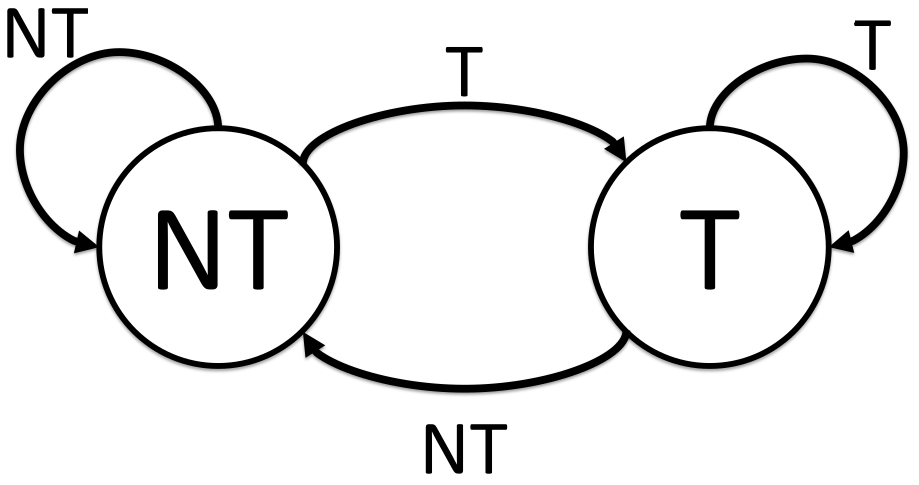
\includegraphics[width = \textwidth]{./images/BHTFSA.png}
								\caption{The NT stands for Not Taken, and T for Taken}
							\end{figure}
							This models the behaviour of the predictor of \emph{which branch is to be taken}.\\
							Important remark: the BHT FSA may \emph{overlap predictions} (in the case for example of nested loops) if the prediction is based on different loops. An enhanced model use a 2-bit register to switch state:
							\begin{figure}[H]
								\centering
								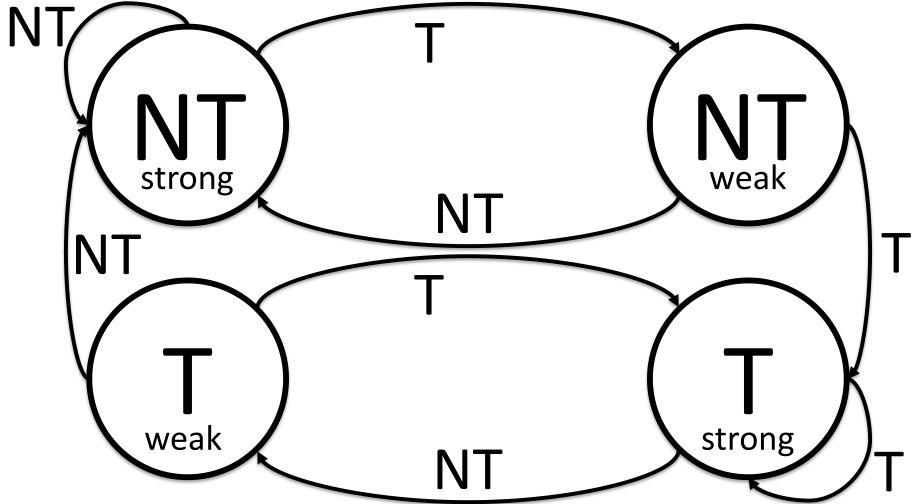
\includegraphics[width = \textwidth]{./images/BHTFSA2.png}
							\end{figure}
							We could also add a third, fourth bit to the memory of the FSA, but sperimental data show that a 2-bit BHT predictor is the best tradeoff between complexity and accuracy.\\
							Another approach is to lenghten the scope of the prediction: what if two threads of execution have a similar pattern in branches, but they're "unlucky"? We could add a dedicated branch predictor that matches previous behaviours with the current one to look for patterns and better decide which path to take. This "multilevel predictors" relies on 2 factors: the lenght of the \emph{behaviour branch} to be analyzed \textbf{and stored} and the number of bits used to discrimine the branch taken (so as the simple predictor: in fact, simple FSA predictors are (0, 2) correlating predictors).\\
							Correlating predictors, in practice, memorize the "story" of a execution path and then feed this story to a normal FSA predictor to compute the outcome.\\
							Even more formally, a $(m, n)$ predictor uses the behaviour of the last $m$ branches to choose from $2^m$ branch predictors, each of which is a $n-bit$ predictor for a single branch. From the implementation point of view, the history of branches is memorized in a shift register of lenght $m$. 
						
						\subparagraph{Branch Target Predictor}
							Simply enough, the BTP is a cache that stores the predicted address to jump to if a branch is taken. It's structured as an hashmap of jump addresses $\rightarrow$ PC-relative jump targets. Every associative entry must also have some validity bits, in order to signal wheter the branch is "in use" or not. Usually, these bits are signaled by the Branch Outcome Predictor.
							\begin{figure}[H]
								\centering
								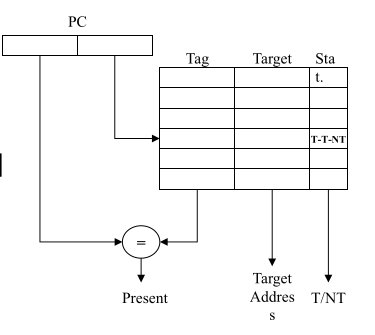
\includegraphics[width = \textwidth]{./images/BTP.png}
							\end{figure}
							
			\subsection{Hazards and Dependences}
				Hazards are hardware issues caused by \emph{code dependences}, that are only related to the instructions to be executed. We can have various type of dependences:
				
				\subsubsection{Name Dependences}
					Name dependences, to be formal, occurs when two instructions use the \emph{same identifier} for a memory location or register, \textbf{but} there's no data flowing between the instructions associated with that name. Careful here: the two instructions does not have a \emph{flow of data between them} does not mean that they're indipendent: they're just sharing a name for a place. If there's no renaming in the architecture, this causes conflicts.
					\begin{itemize}
						\item Antidependences: an instructions write data in a named space that a following instruction will read (if not managed, this causes WAR hazard, but remember: hazards are pipeline properties, dependences are program properties)
						\item Output dependence: two instructions write data in the same named location (WAW)
					\end{itemize}					
					
				\subsubsection{Data Dependences}
					True data dependences are the classic logic dependences that cause RAW hazards.
				
				\subsubsection{Control Dependences}
					Control dependences are those relationships among instructions that must be executed after a control operation that can vary the program flow.
						
	\clearpage \part{Parallelism}
		\section{Instruction Level Parallelism}
			"Potential overlapping of of execution among unrelated instructions". This definition of parallelism includes pipelined architectures: in fact, at every clock cycle, a pipeline is executing a number of instructions that's up to the number of stage it's composed of. \emph{Actual} parallelism can be achieved by parallel architecuters (so hardware that is designed to handle multiple instructions per clock cycle) such as superscalar architecures and VLIW.\\
			ILP is \emph{not} parallel processing! The first is just pipeline operations to enhance throughput, the second is a non-user-transparent way of \emph{executing programs}.\\
			ILP is possible $\Leftrightarrow$ there are no WAR, WAW, RAW conflicts, neither strtuctural hazards or control stalls.\\
			At first, we must introduce the Complex Pipeline in order to understand the aim of the procedures to implement ILP. 
			
			\subsection{Complex Pipeline}
				The complex pipeline has multiple path between the DECODE step and the WRITE BACK phase. This means that \emph{right after} the decode phase an additional phase (called "issue") that send the operation to the correct pipeline must be introduced. The complex pipeline \emph{does not create real parallelism between instructions} because in any case the EXE stage will not be shared among instructions. It just introduces the problem of having to deal with \emph{multiple data path} that each introduce a potential critical path to the architecture. Each one of those additional datapath can have a different clock count (an integer operation could take less than a "load word" operation, in terms of clock cycles) and thus enhance throughput. This, however, could lead to problems in the fetch phase of operations.\\
				A possible solution (in fact, the superscalar once) is to load two instructions per clock cycle, and send them down different paths if they're "different" (basing on the dedicated hardware for each). The additional assumption is, every alternative EXE path is delayed in order to have a homogeneous clock cycles number before the WB stage.
				\begin{figure}[H]
					\centering
					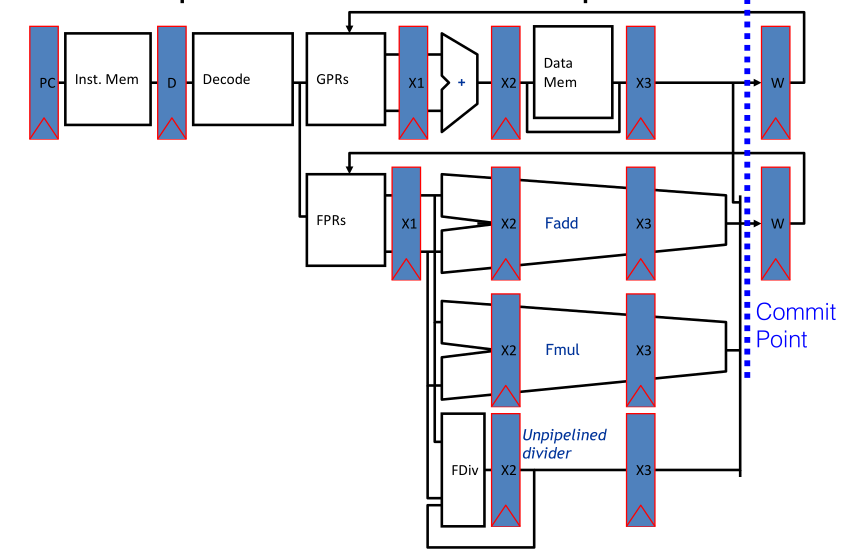
\includegraphics[width = \textwidth]{./images/complexPipeline.png}
					\caption{Here we see how the three different EXE stages are delayed-stalled all to match the longest data path (the FAdd, FMul one)}
				\end{figure}
				
			\subsection{VLIW}
				Very Long Instruction Word allows actual parallelism between instructions. This is done with the aim to raise the CPI above one $\Rightarrow$ having multiple instructions completed \emph{simultaneously}. The idea is to delegate the scheduling of the operations \emph{entirely} to the compiler, and enable the processor to fetch more than one operation per cycle. To do so, an additional distinction between instrutions and operations is needed:
				\begin{itemize}
					\item Operation is the basic unit of computation
					\item Instruction is a batch of operations; all the operations in the batch can be executed simultaneously
				\end{itemize}
				The compiler now has to arrange operations in these batches (the VLIW instructions) that (due to their dimension) justify the name "Very Long Instruction". The Fetch, Decode, Mem and Write Back phases are unchanged in these architectures, juste the EXE block is replicated and parallelized.
				
				\subsubsection{Enforcing ILP}
					In a regular program, it's difficult to find parallel-prone batches of instruction. The compiler has to figure out how to enhance code translation in order to fully use the parallel architecture underneat.
					
					\paragraph{Loop Unrolling}
						A simple example is the way loops that access sequential (or random access) data structure, just as a simple foreach, can be "unrolled", so more iteration of it can be executed at the same time. N.B.: this must be compatible with the conflicts in the code!
						
					\paragraph{Software Pipelining}
						In order to enhance Loop Unrolling performance, again rescheduling comes in hand. In which way? Basically "anticipating the next loop iteration" at a scheduling level. This is made by anticipating operations \emph{in order to free slots in the pipeline that can be used to startup next iterations}. It's probable that some "compensating instructions" must be added.\\
						We can see Software Pipelining as a Loop Unrolling \emph{enhanced} because it's just LU that pays the "startup" and "wind down" operation \emph{just one time per loop} instead of \emph{once per iteration}.
						\begin{figure}[H]
							\centering
							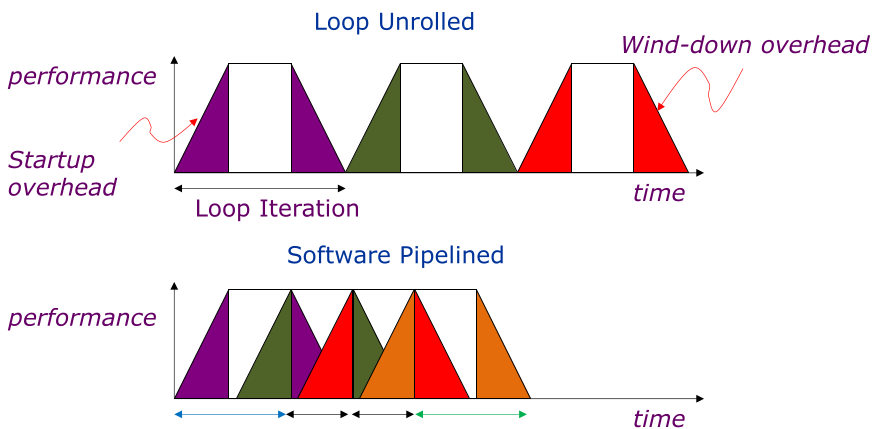
\includegraphics[width = \textwidth]{./images/swpipe.png}
							\caption{Visualization of the improvement of Software Pipelining}
						\end{figure}
						REMEMBER: SP is a \emph{compiler} solution, that just \emph{exploits efficently} a VLIW architeture.
					
					\paragraph{Trace Scheduling}
						A trace is a loop free sequence of basic blocks (of instructions) embedded in the control graph. It's an "execution path" for the application. The idea behind trace scheduling is to execute application and profile the traces (against fixed input) to find the \emph{most probable to be executed}. Then, consider the entire string of "probable blocks" as a single one, in order to apply heavy rescheduling to the whole operations set, to enhance performance.
						
					\paragraph{Messing with Code}
						Compensating code (like decreasing a counter afterwards having anticipated the increment) can be super cool when it comes to rescheduling operations in order to exploit hardware parallelism. BUT it must be handled with care, just like rescheduling \emph{itself}. There are some well estabilished techniques:
						\begin{itemize}
							\item Speculative execution: "move around" code that we \emph{think} (probabilistically) can be executed.
							\item Predicated execution: we use the parallelization at the hardware level to simultaneously execute different branches of a conditional block and then \emph{validating} only the right one.
						\end{itemize}
						
		\section{Dynamic Scheduling}
			So, dynamic scheduling is the procedure to "rearranging instructions/operations" in order to fully exploit the hardware. Keep in mind that we're talking about \emph{hardware solutions} to reschedule operations, so the additional hardware needed to analyze instructions, look for dependencies and dispatch executions increases (significantly) the overall complexity of the architecture.
			
			\subsection{Scoreboard}
				\subsubsection{Scoreboard Data Structures}
 					In order to properly manage the complex pipeline and "give the right timing" to each instructions, functional unit and register, the scoreboard architecture makes use of additional data structures. The most important is a "hash map"-like stucture that links every functional unit to a set of flags and pointers, in detail:
 					\begin{enumerate}
 						\item A \emph{busy} flag that signals wheter the FU is in use
 						\item A \emph{op} vector that describes the available operation in that FU. This is also used to \emph{tell multi functional units which is the desired operation}
 						\item Three pointers to the registers (one for the destination, two for the sources, obviously)
 						\item Two pointers to the functional units that \emph{should produce the desired value} (this pointer is used to detect RAW conflicts) and that is linked to the source/destination register pointer (in fact, if we call $F_i$ and $F_j$ the two source registers, these two pointers would be $Q_i, Q_j$). More than pointers, this are FU ids, like "integer module 1" or "adder 2"
 						\item Two additional flags ($R_j, R_k$) that signals \emph{when} $F_j,F_i$ are ready. These two bits are used \emph{alongside the other flags and pointers} to signal if the instruction is waiting for data, but their meaning changes depending on the type of instruction and the phase of it
 					\end{enumerate}
 					This hashmap (which index is the FU) is called \emph{functional unit status} and works with an additional array of signals the status of all registers, the \emph{register result status}.
					\begin{figure}[H]
						\centering
						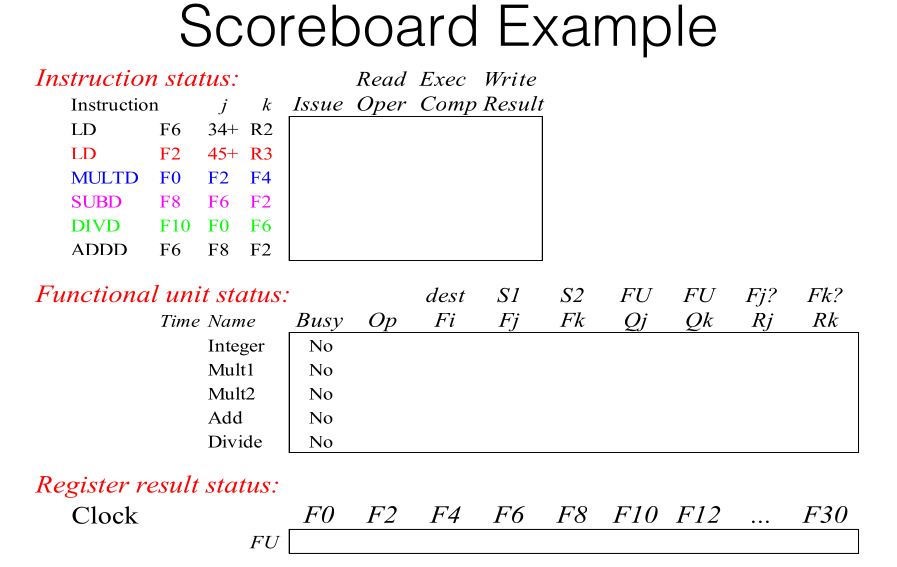
\includegraphics[width = \textwidth]{./images/Scoreboard1.png}
						\caption{The scoreboard blank data structures}
					\end{figure}
			 		\begin{figure}[H]
						\centering
						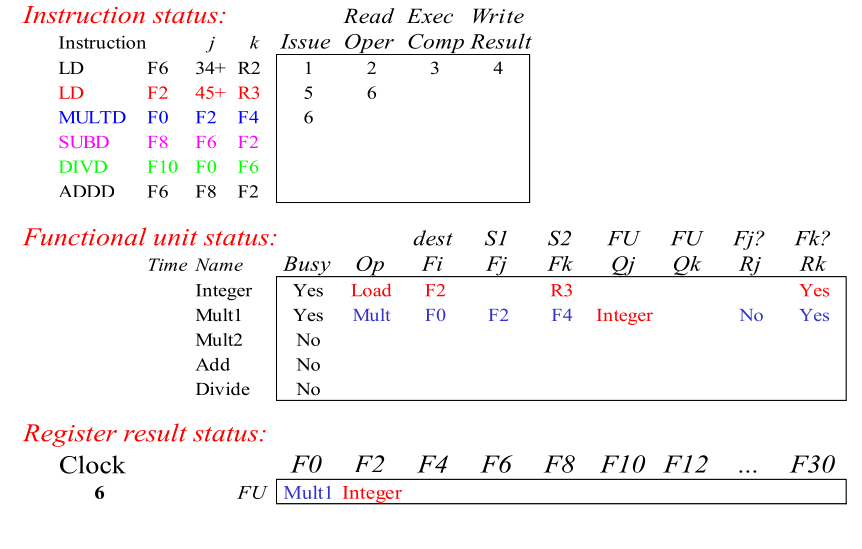
\includegraphics[width = \textwidth]{./images/Scoreboard2.png}
						\caption{The scoreboard data structures executing an instruction}
					\end{figure}
			
			\subsubsection{Scoreboard - The Algorithm}
				Environment: complex pipeline with "ISSUE" stage, we need to implement out of order execution. The basic solution is to split the ID stage in two, the first that analyzes the instruction and the second that \emph{computes the operands and detects hazards}. An instruction is allowed to fire if there are no hazards. \textbf{So if instruction 2 follows instruction 1 and the latter is blocked due to an hazard \emph{but 2 is free to fire}, 2 will execute normally}.\\
				That means that a scoreboard dynamic scheduled pipeline is
				\begin{itemize}
					\item In order issued
					\item out of order executed
					\item out of order committed (writebacked)
				\end{itemize}
				
				The Scoreboard pipeline is ultimately divided in 4 main stages:
				\begin{enumerate}
					\item The issue stage decodes the instruction and detects the hazards. Instructions are issued in program order. Stalling this phase is used to avoid WAW and structural hazards, and it's done if 
						\begin{itemize}
							\item There's not a functional unit ready for this type of operation
							\item There's a conflict in the target register
						\end{itemize}
						If no hazards are detected, the Read Operands stage is entered
					\item Due to the fact that there's no possible forwarding in this pipeline, scoreboard hardware needs to tell each FU when it can read from registers. This is the stage to be stalled in order to avoid RAW hazards. An instruction is stalled here if one (or both) of its $R_i$ is set to false.
			 		\item Execution stage: the FU gets the operands when the scoreboard enables the Read Operands stage "right behind" the exe stage, and this stage notifies the scoreboard when the result is ready. The execution phase can take up different amount of clock cycles based on the kind of operation performed.
		 			\item Accessing to the registers in order to write back the results of instructions execution. This stage can be stalled if a WAR is detected.
 				\end{enumerate}
 				Ultimately, the Scoreboarding approach removes RAW hazards, by \emph{issuing an operation only when its operands are available}, and WAR hazards, by \emph{stalling the writeback phase if needed}. WAW hazards are still to be taken care of.
 				
 				
					
			\subsection{Tomasulo Algorithm}
				Tomasulo algorithm is a dynamic algorithm that enables out of order execution and out of order completion for instructions (issuing is still handled in order). The goal of this algorithm is the same of scoreboard: high performance without compiler intervention. The main difference between Tomasulo and Scoreboard is how the control logic is handled: in Scoreboard is centralized, while in Tomasulo approach are distributed and \emph{nearer} to the functional units. Operand buffers are called \emph{reservation station}. Tomasulo's architectures resolves WAW and WAR hazards efficiently by exploiting \emph{register renaming}.
				\begin{figure}[H]
					\centering
					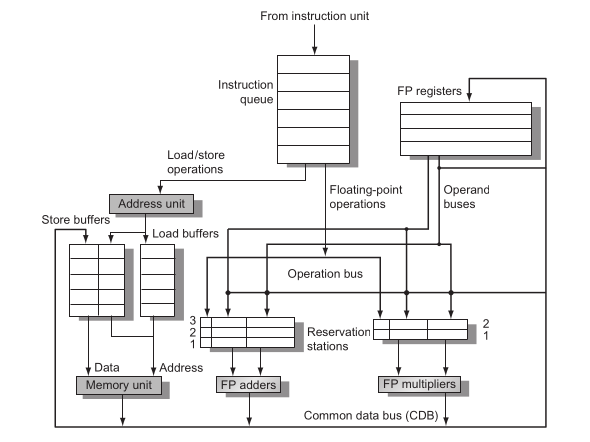
\includegraphics[width = \textwidth]{./images/TomasuloArchitecture.png}
					\caption{Basic Tomasulo architecture}
				\end{figure}
				
				\subsubsection{The reservation stations}
					The reservation stations are the core of the Tomasulo mechanism. They're the buffer between the register file and the actual functional units, and \emph{embody the register renaming approach} that lies under the Tomasulo algorithm. Also, proxies are introduced for the "load from memory" operations (load buffers) and for the write back operations (store buffers).\\
					The reservation stations can access a common data bus (the hearth and nervous system of the Tomasulo architecture) that makes available / read the values broadcasted from Reservation Stations.
					
				\subsubsection{Tomasulo data structures}
					Tomasulo decentralized approach does not affect much the kind of information needed in solving this problem. In fact, the \emph{very same information} is just scattered near the functional units, inside the reservation station. The reservation station, in fact, are made up of:
					\begin{itemize}
						\item A string indicating the type of operation needed
						\item $V_j$ and $V_k$ the values of the source operands (value = copies)
						\item $Q_j$ and $Q_k$ pointers to the reservation station that produces $V_j$ and $V_k$. Can be used to \emph{bypass} $V_j$ and $V_k$ 
						\item a "busy" flag
					\end{itemize}
					
			 	\subsubsection{Three stages Tomasulo architecture}
					The Tomasulo pipeline is divided in
					
					\paragraph{ISSUE stage}
						Get the instruction from the queue and if a RS is ready, \emph{set the right values of it}, that can be either in the registers or in a issued computation; in the latter case, the pointers to the FU that will produce the right value are given to the issued intruction. If there's no station available, the operation is stalled: we're in presence of a structural hazards. In this step registers are renamed, avoiding WAR and WAW hazards.
					
					\paragraph{EXECUTION stage}
						If an operand is not ready \emph{it will arrive from the shared data bus}. In this stage operands are "waited" monitoring the CDB, and each RS and FU knows which other will produce the desired value because of the ISSUE stage providing thi information earlier.
						
					\paragraph{WRITE stage}
						In this phase the result of the FU computations are broadcasted on the common data bus and stored in the RS that requested it and in the Store Buffers, in order to be stored in memory or in the RF eventually.
						
	\clearpage \part{Interrupts and Exceptions + Handling}
		\section{Interrupts}
			An interrupt is a "signal" that alter the normal control flow of a program, \emph{at runtime}. An interrupt must be handled by a dedicated \emph{interrupt handler} and then the architecture should be able to \emph{resume the normal execution of the program}. An interrupt can come from the program that's executing as well as the external environment. An ACA definition of an interrupt is "an event that requests the attention of the processor". We can characterize interrupts in a super complicated way:
			\begin{enumerate}
				\item A/Synchronous
				\item User requested or coerced
				\item User maskable or unmaskable
				\item Within or between instructions
				\item Resume/Terminate events
			\end{enumerate}
			
			\subsection{Asynchronous Interrupts}
				Hardware signals, timer expirates are all async interrupts. They're all caused from external sources instead of the currently running program. These kind of interrupts can be handled at the end of the execution of the current instruction, and thus they're far easy to manage wrt sync interrupts.
				
				\paragraph{The Interrupt Handler}
					When an external interrupt is invoked (an I/O change, for example) the CPU should switch the context of the execution from the currently executing program to the code of the interrupt handler, the piece of code that carries out the managing of the event. So all the instruction up to $I_i$, so $I_{i-1}...$ must be completed (this defines a precise interrupt, also\footnote{An interrupt is said to be precise if an istant can be identified so that all instruction before that moment can commit their state and no subsequent (to the interrupt) instruction modifies the saved state. Precise interrupts are desiderable because (obviously) \emph{execution can be resumed easily} and because they generate a "safe state" to proceedback from.}), the PC must be saved and the execution must be transferred to a dedicated kernel-level interrupt handler. 
				
			\subsection{Synchronous Interrupts}
				Synchronous interrupts (also called \emph{exceptions}) are interrupts and errors generated by the curently running program. Undefined opcode, program error (zero division) or misaligned memory are all interrupts that come from the running program itself. These exceptions are rare, but they're problems, and they must be handled carefully.\\
				A synchronous interrupt is caused by a particular instruction (so generally is a \emph{within instruction} kind of interrupt) and generally cause the instruction itself (if not the entire routine) must be restarted. 

		\section{How to Handle Interrupts in a Five Stage Pipeline}
			For each stage of a pipelined architecture, additional hardware must be deployed in order to catch interrupts and handle them. This is due to the fact that every stage can cause errors: arithmetic faults are caused by the ALU, wrong opcodes are catched in the first stage, memory errors are generated in the last one and so on.\\
			A valid method is to add a flag to the instructions that signals wheter that instruction has caused an excepion or not. Interrupts-generating instructions are then NOPped and the pipeline flushed. The next instructions to be fetched are the ones of the interrupt handler. In which order are exceptions handled? If we wait till the last pipieline stage (the commit point) and then we collect the exceptions flag and execute the handlers \emph{in order} we solve the problems related to have multiple parallel instructions faulting at the same time.

	\clearpage \part{Superscalar Architectures}	
		\section{Superscalar Approaches}
			"Why not fetch multiple instructions at the same clock cycle?"\\
			Superscalar architectures do exactly this: they enable the fetch unit to retrieve more instructions per clock cycle (theoretically we have a CPI < 1!) and make extensive use of register renaming, dynamic scheduling and dynamic branch prediction techniques in order to avoid data hazards.
			\begin{figure}[H]
				\centering
				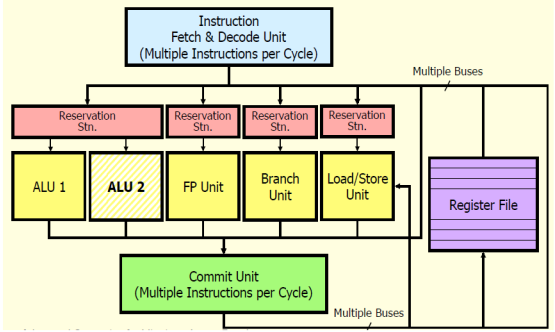
\includegraphics[width = \textwidth]{./images/superscalar.png}
				\caption{A classic superscalar microarchitecture. Note the resemblance with a classic Tomasulo-like processor.}
			\end{figure}
			
		\section{Limits of ILP Exploiting}
			Instruction Level Parallelism cannot be squeezed beyond a certain point.
			\begin{enumerate}
				\item Dynamic scheduling is very expensive, and also very hard to design and to verify
				\item Register renaming also has its limits: using a bottomless buffer for names is not a realistic idea, and ultimaltely does not resolve all conflicts
				\item Jump and branch predictions are not 100\% accurate
				\item We have still to deal with latency in memory
				\item In case of superscalar architectures, we cannot issue \emph{too many} instructions at the same time: we still have to deal with hazards
			\end{enumerate}
			Summing up: ILP has an upper bound. This upper bound is dependant \emph{surely} on the technology we use to implement CPUs, but not only: it is influenced by the complexity inherent in the executing of multiple instructions at the same time, considering overlaps, jumps, conditional jumps, exceptions. All these aspects must also take into account power consumption (technological barrier: still a relevant issue) and design complexity.\\
			Here, at the top of the upper bound of ILP exploitation, we can see the real limit of SISD architectures. We should look further to different type of architectures in order to increase performance again.
			
	\clearpage \part{Multiple Cores}
		\section{How to Handle Explicit Parallelism}
			Ok so, we reached ILP. We next step is to introduce \emph{real} parallelism (\emph{explicit parallelism}). As usual, multiple models can be adopted in order to introduce parallelism into the process model:
			\begin{enumerate}
				\item Single process single thread: no parallelism
				\item Single process multiple threads
				\item Multiple process single thread
				\item multiple processes multiple threads
			\end{enumerate}
			Obviously, switching between two processes is heavier than switching between two threads. 
			
			\subsection{Multithread Single Core Architectures - Multiprocessors}
				To introduce real parallelism in a non-parallel architecture, we must rely on a super fast control unit that handles a lot of thread-context-switches at a time. Assuming this kind of CU exists, how thread can interleave in a pipeline? 
				
				\paragraph{Temporal Multithreading}
					An architecture that exploits temporal multithreading uses the processor for a single task at a time. The parallelism is put in place by switching between tasks \emph{over time} and \emph{preemptively}, in roder to give the illusion of parallelization. This is not really hardware multithreading, because the maximum number of tasks (processes, threads) in execution at the very same time is always one.\\
					We can distinguish between:
					\begin{enumerate}
						\item Fine grain parallelism: each \emph{instruction} is followed by another thread \emph{instruction}. This hides short and long stalls, because a stalled thread "leaves the pipeline free" for another thread. 
						\item Coarse grain parallelism: switch between threads only when a long stall is asked from a thread. This enables the threads to interleave in a more efficent way. 
					\end{enumerate}
				
				\paragraph{Simultaneous Multithreading}
					Can we exploit ILP methodologies to enhance parallelization instead of single-thread-throughput? Yes; \emph{simultaneous multithreading}. We can use a superscalar architecture to fetch instruction \emph{from different indipendent threads} when loading instructions; this is made possible by keeping track of two (or more) different program counters. BUT this is not a real limitation, because we can make large use of register renaming. Moreover, the intrinsic OOO execution of the tasks in a superscalar processor allows threads to execute in real parallelism.\\
					Actually, SMT (alongside pure multiprocessing, where the CPU is "split in lanes" that executes each a thread per time) implements hardware parallelism.
					
				\paragraph{Comparison of approaches}
					\begin{figure}[H]
						\centering
						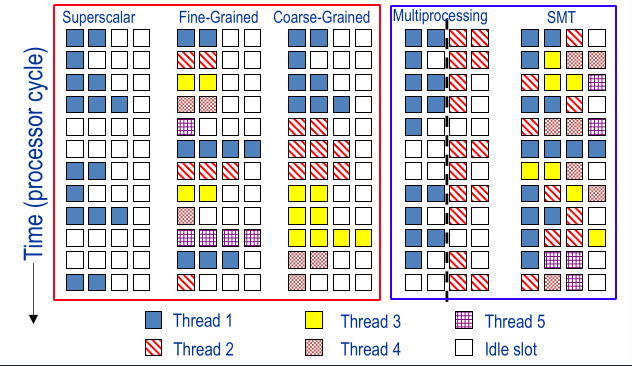
\includegraphics[width = \textwidth]{./images/threadLevelParallelism.png}
						\caption{In red, temporal multithreading approaches. In blue, simultaneous multithreading approaches.}
					\end{figure}
					Without surprise, temporal multithreading is not as "thoughtputful"\footnote{completely made up on the spot} as simoultaneous multithreading, being the second an actual \emph{hardware} multithreading approach, with more process simoultaneously on the same chip.\\
					This is due also to the fact that fetching instructions from multiple threads enables to always execute the best candidate (basing on the number of unresolved branches, load misses ecc) to execute, and thus committing more instructions. \emph{As usual}, a more "intelligent" architecture is also more difficult to design: having to deal with
					\begin{enumerate}
						\item Multiple executions contexts
						\item Multiple fetch candidates
						\item Cross thread commit conflicts
					\end{enumerate}
					add complexity to the hardware (that drives more power consumption ecc ecc).
					
		\section{Parallel Architectures}
			As a formal definition of a parallel computer is a "set of computers that can \emph{cooperate and communicate} to solve a problem". In this definition is made relevant that the \emph{communication infrastructure} of a parallel architecture is one of the performance indicator for it. An architecture can achieve single core performance like no other, but if the communication infrastructure is poor this power is thrown away.\\
			We can have at least three models of parallelisms (according to Flynn's taxonomy, SIMD, MISD, MIMD). The first parallel architectures (the '80) were \emph{parallel SIMD architectures} and were used for vector computations. MIMD is the "way to go": if we can achieve real parallelism on-chip \emph{on multiple data} we will have an higher processing per chip ratio (to say one).
			
			\subsection{SIMD}
				First in the list of parallel architectures, single instruction stream on multiple memory units (vector computation).
				\begin{figure}[H]
					\centering
					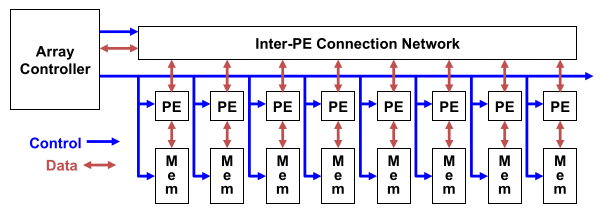
\includegraphics[width = \textwidth]{./images/SIMD.png}
					\caption{A traditional SIMD computation, with a central arbiter that delivers to each \emph{processing element} the same instructions to execute \underline{on their private memory}}
				\end{figure}
				SIMD architectures can be seen as an orchestra made of an array of a unique instrument, all the intruments playing the same note at the same time.\\
				Vector computation is peculiar in the sense that each processing element (each instrument in the orchestra) must have his memory space; this leads to a "vectorized" architecture \emph{on more levels}: also registers must be vectorized, buses and I/O ports. Even more: loop unrolling can be easily performed when a VISA is available: an entire loop can be summed up in a single vector instruction (if iterations are indipendent) saving up a lot of time; a single instruction is neede instead of a loop. 
				
				\paragraph{Vector ISAs}
					To deal with vectorized architectures, we also need \emph{vector instructions} that can deal with multi-dimensional memory and processing elements. A VISA is compact (bundles together several operations in a single instruction) and scalable (just add lanes!). It is also super expressive: a single vector instruction not only bundles together multiple operations, but also "means more" in terms of memory access, data dependancy and independency between operations. As an example, MIPS-like code comparison for a simple sequential pipeline loop and a vectorized architecture:
					\begin{figure}[H]
						\centering
						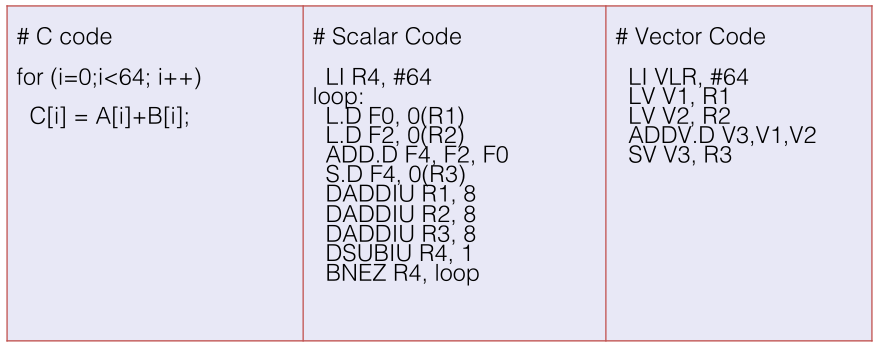
\includegraphics[width = \textwidth]{./images/vISAs.png}
					\end{figure}
					It's obvious that not every cycle will be exactly as long as the vector lenght: to ensure that the vector architecture is fully exploited, two techniques are used:
					\begin{enumerate}
						\item Strip mining: assembly code is generated in a way that every cycle is unrolled (but more in general, every operation is generate as) to always fit the \emph{mvl}\footnote{maximum vector lenght} and no further. A vectorized loop handles all the multiple-of-mvl long operations and then a scalar clean-up loop handles the remaining part of the data. 
						\item Vector mask control: when for example a loop contains operations on data that depends on a condition (like, increment only odd values of an array) an array of boolean values is generated and only the flagged generated data are then transcribed in the register file. 
					\end{enumerate}
					
			\subsection{MIMD}
				MIMD architectures pushes heterogeneous approaches. Why? Because having multiple instructions executing at the same time on different data means that potentially perform super different computations \emph{at the same time on the same chip}. The perfect example is mobile multi purpose devices, that have to handle a ton of computations at the same time that are not \emph{so computationally expensive}, but they're all different from one another: text processing lives besides video processing and communications.\\
				MIMD processors are arrays of processors that work asynchronoulsy on different data. Little detail: this vague definition of MIMD machines includes parallel omogeneous architectures as well as heterogeneous chips and also clusters of indipendent machines.\\
				
		\section{Classes of MIMD Machines and their Memory Models}
			We can classify MIMD machines either by the address space model or the physical implementation of the memory itself:
			\begin{itemize}
				\item single shared address space memory architectures, where all processors share the same memory addresses\footnote{\emph{NOT THE SAME MEMORY, but only the addressing space. Can be the same memory though.}}(it's usually up to the OS to maintain coherence). This solution provides low overhead: there's no difference for a process to load data from memory and passing data to another process. On the other hand, the management of the address space is a mess. Also, it does not scale well.
				\item multiple private address spaaces, in which every processor access his own memory. Usually this kind of architectures provides send/receive primitives to enaable data sharing, through some implementation of a message passing protocol. 
			\end{itemize}
			for the address space, and
			\begin{itemize}
				\item Centralized shared memory architectures, where cores\footnote{better if not too many, max 100} share the same physical memory banks. These archs are usually called Uniform Memory Access.
				\item Distributed memory architectures, where each core has his own main memory. These solutions often need a high bandwith interconnection, but usually can support more cores. Are usually called NUMA (Non Uniform Memory Access).
			\end{itemize}
			for the physical memory implementation. This model cohesists: to cite professor Santambrogio: \emph{The concepts of addressing space (single/multiple) and the physical memory organization (centralized/distributed) are orthogonal to each other}.
			\begin{figure}[H]
				\centering
				\begin{minipage}{0.45\textwidth}
					\centering
					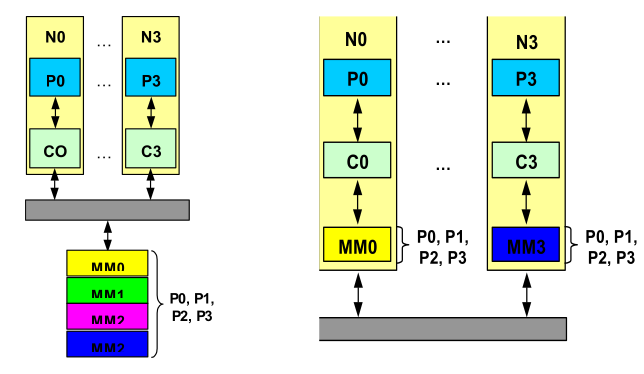
\includegraphics[width=0.9\textwidth]{./images/sharedMemory.png}
					\caption{Shared address space architectures: centralized memory vs distributed memory}
				\end{minipage}\hfill
				\begin{minipage}{0.45\textwidth}
					\centering
					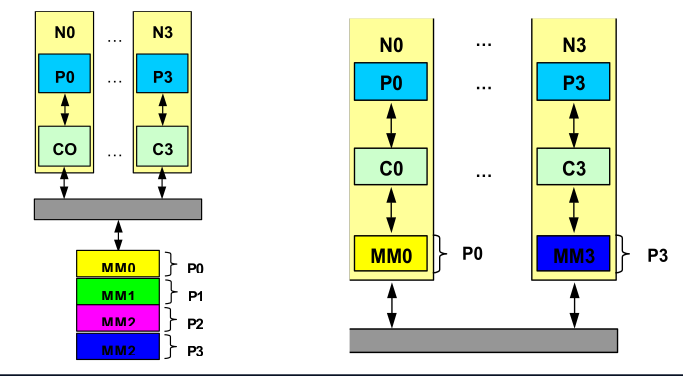
\includegraphics[width=0.9\textwidth]{./images/messagePassing.png}
					\caption{Message Passing architectures: centralized memory vs distributed memory}
				\end{minipage}
			\end{figure}
			This kind of shared vs indipendent models can be also seen in the programming model that finally ends up in the developer hands. However, \emph{every programming model} can be implemented on top of \emph{every kind of architecture}.
			
			\paragraph{Reference Model}
				For all the subsequent examples, we'll use a Bus Based Symmetric Shared Memory system:
				\begin{itemize}
					\item Bus Based: all processing units share a communication media that's uniform (and easy to monitor)
					\item Symmetric: all processing units are "equal" with respect to the bus
					\item Shared Memory: every processor access the same memory through the bus itself.
				\end{itemize}
				The key improvement to this model (also, the one we'll consider) adds caches to the processing units. These can be organized and manaaged to be coherent with the central memory by the hardware itself. 
			
			\subsection{Shared Memory Problems - Coherence}
				Coherence in memory can be seen as the problem to maintain the property "any read on a block must return the most recently written value on that block". This plain concept is crazily difficult to implement, so it turned in a serialization property. The core idea behind memory coherence is that every processing unit should not read data that's outdated. "Memory coherence" itself contains two concepts:
				\begin{itemize}
					\item Coherence itself: this term refers to which value should be returned by a read
					\item Consistency: determines \emph{when} the effect of a write can be seen by other units
				\end{itemize}
				From the Patterson Hennessy: \emph{Coherence and consistency are complementary: Coherence defines the behavior of reads and writes to the same memory location, while consistency defines the behavior of reads and writes with respect to accesses to other memory locations}.\\
				Before digging into consistency protocols, we need two basic definitions for writing policies:
				\begin{enumerate}
					\item Write back caches hold the updated value in the cache until an explicit flush is called
					\item Write through caches immediatly flush the updated value to the main memory on a write operation
				\end{enumerate}
				Now, consistency protocols: there are plenty of solutions to enforce consistency and coherence in memory hierarchies, we'll se Snooping Protocols.
				
				\subsubsection{Snoopy Bus}
					The bus is intrisecally a broadcast communication medium between all processing units. This suggests the PU to monitor it looking for changes, and to be able to understand when a cached value is not anymore valid. These protocols can be divided in two main categories, depending on what happens when a write operation is issued.
					
					\paragraph{Write Invalidate}
						Write Invalidate protocols add an "invalidate" signal to the write operation: this tells all other units attached to the bus that they have an outdated value for the written memory block. All processors will now fetch the updated value from the main memory \emph{on their own}. 
					
					\paragraph{Write Update}
						The fat brother of Write Invalidate is Write Update: "update all values in all caches when a write operation is performed". Fat because logically it needs much more bandwidth that WI.
						
					\paragraph{MSI}
						Modified Shared Invalid protocol: the funtioning of this protool is explaind by the automaton
						\begin{figure}[H]
							\centering
							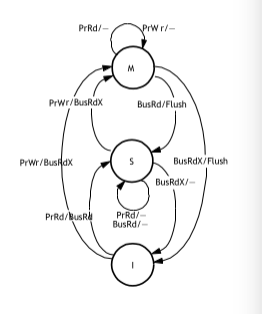
\includegraphics[width = \textwidth]{./images/MSI.png}
						\end{figure}
						This simple protocol marks the cache blocks with different labels and acts accordingly. This approach is shared by all consistency protocols: a cache block has a state associated that evolves as the automaton says.
						
					\paragraph{MESI}
						MESI is MSI plus the Exclusive state, which is inserted in the automaton this way:
						\begin{figure}[H]
							\centering
							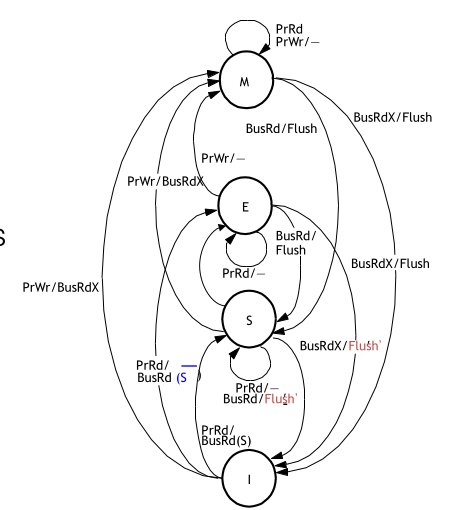
\includegraphics[width = \textwidth]{./images/MESI.png}
						\end{figure}
				
		\section{GPUs}
			When talking about heterogeneous architectures, we cannot avoid thinking about dedicated hardware, and GPUs are the best example. The gaming (and physics) industry carried the developing of processing units that were \emph{dedicated} to graphical processing, to speed up execution for example in games, or simulators.
			
			\subsection{Procedural Synthesis}
				Procedural synthesis is a method to \emph{generate content} dynamically basing on random or pseudo random seeds. This technique is used to generate for example low level geometry for landscape in videogames. In this very case, objects are composed of polygones that are stored in memory as set of vertices.
				
				\paragraph{XBox 360's Solutions to Procedural Synthesis}
					Xbox 360 by Microsoft uses this workflow to render scenes of videogames:
					\begin{enumerate}
						\item Store in the main memory high level descriptions of the objects to render.
						\item Use the CPU to carry out the procedural synthesis of the \emph{geometry} at runtime, to create the skeleton of the scene.
						\item Use the GPU to load then the graphic components such as textures, and put together the full scene.
					\end{enumerate}
			
			\subsection{GPUs and CPUs}
				Architecturally, GPUs are completely different from standard CPUs. While CPUs are oriented to serial execution of instructions, GPUs are more tailored to highly parallel execution to achieve higher volumes of computation.
				
			\subsection{The GPU Pipeline}
				The GPU work is to receive geometry as input and produce an image corresponding to that geometry as an output. This is made possible through the workflow
				\begin{enumerate}
					\item interface with the host: this stage of the pipeline gets the information (so vertices) from the CPU and the other main geometry infos (vectors and stuff).
					\item vertex processing: in this stage all the vertices are connected to form the right shapes. 
					\item triangle setup: all the forms outputted from the vertex processing stage are processed in order to realize \emph{which portions of which geometry elements} should be mapped on the final figure.
					\item pixel processing: all the textures are applied in this portion of the pipeline.
					\item last stage: memory interface. 
				\end{enumerate}
				
		
			
\end{document}
